\chapter{Planning for \LTLf/\PLTL Goals}\label{ch:planning}
In this chapter, we will define a new approach to the problem of non-deterministic planning for extended temporal goals. In particular, we will give a solution to this problem reducing it to a fully observable non-deterministic (\FOND) problem and taking advantage of our tool \LTLfToDFA, presented in Chapter \ref{ch:ltlf2dfa}. First of all, we will introduce the main idea and motivations supporting our approach. Then, we will give some preliminaries explaining the Planning Domain Definition Language (\PDDL) language and the \FOND planning problem formally. After that, we will illustrate our \FONDFOR approach with the encoding of temporal goals into a \PDDL domain and problem. Finally, we will present our practical implementation of the proposed solution.
\section{Idea and Motivations}\label{sec:plan-idea-motiv}
Planning for temporally extended goals with \textit{deterministic} actions has been well studied during the years starting from \citep{bacchus1998planning} and \citep{doherty2001talplanner}. Two main reasons why temporally extended goals have been considered over the classical goals, viewed as a desirable set of final states to be reached, are because they are not limited in what they can specify and they allows us to restrict the manner used by the plan to reach the goals. Indeed, temporal extended goals are fundamental for the specification of a collection of real-world planning problems. Yet, many of these real-world planning problems have a \textit{non-deterministic} behavior owing to unpredictable environmental conditions. However, planning for temporally extended goals with \textit{non-deterministic} actions is a more challenging problem and has been of increasingly interest only in recent years with \citep{camacho2017non, de2018automata}.

In this scenario, we have devised a solution to this problem that exploits the translation of a temporal formula to a \DFA, using \LTLfToDFA. In particular, our idea is the following: given a non-deterministic planning problem and a temporal formula, we first obtain the corresponding \DFA of the temporal formula through \LTLfToDFA, then, we encode such a \DFA into the non-deterministic planning domain. As a result, we have reduced the original problem to a classic \FOND planning problem. In other words, we compile extended temporal goals together with the original planning domain, specified in \PDDL, which is suitable for input to standard (\FOND) planners.
\section{Preliminaries}
In this section, we will give some basics on the \PDDL specification language for domains and problems of planning and a general formalization of \FOND planning.
\subsection{\PDDL}\label{sec:pddl}
As stated before, \PDDL is the acronym for Planning Domain Definition Language, which is the \textit{de-facto} standard language for representing ``classical'' planning tasks. A general planning task has the following components:
\begin{itemize}
\item Objects: elements in the world that are of our interest;
\item Predicates: objects properties that can be true or false;
\item Initial state: state of the world where we start;
\item Goal state: things we want to be true;
\item Action/Operator: rule that changes the state. 
\end{itemize}
Moreover, planning tasks are composed by two files: the \textit{domain} file where are defined predicates and actions and a \textit{problem} file where are defined objects, the initial state and the goal specification.
\subsubsection{The \textit{domain} file} 
The \textit{domain} definition gives each domain a name and specifies predicates and actions available in the domain. It might also specify types, constants and other things. A simple domain has the following format:
\begin{lstlisting}[language=PDDL, escapechar=£, label={code:pddl-domain}]
(define (domain DOMAIN_NAME)
  (:requirements [:strips] [:equality] [:typing] [:adl] ...)
  [(:types T1 T2 T3 T4 ...)]
  (:predicates (PREDICATE_1_NAME [?A1 ?A2 ... ?AN])
                (PREDICATE_2_NAME [?A1 ?A2 ... ?AN])
	       ...)

  (:action ACTION_1_NAME
    [:parameters (?P1 ?P2 ... ?PN)]
    [:precondition PRECOND_FORMULA]
    [:effect EFFECT_FORMULA]
   )
  (:action ACTION_2_NAME
    ...)
  ...)  
\end{lstlisting}
where \texttt{[]} indicates optional elements. To begin with, any \PDDL \textit{domain} definition must declare its expressivity requirements given after the \texttt{:requirements} key. The basic \PDDL expressivity is called \textsc{strips}\footnote{\textsc{strips} stands for STanford Research Institute Problem Solver, which is a formal language of inputs to the homonym automated planner developed in 1971.}, whereas a more complex one is the Action Description Language (\textsc{adl}), that extends \textsc{strips} in several ways, such as providing support for negative preconditions, disjunctive preconditions, quantifiers, conditional effects etc.. Nevertheless, many planners do not support full \textsc{adl} because creating plans efficiently is not trivial. Although the presence of this limitation, the \PDDL language allows us to use only some of the \textsc{adl} features. Furthermore, there are also other requirements often used that can be specified as \texttt{equality}, allowing the usage of the predicate \texttt{=} interpreted as equality, and \texttt{typing} allowing the typing of objects. As we will explain later in Section \ref{sec:planning-implementation}, our practical implementation supports, for now, only simple \textsc{adl}, namely conditional effects in domain's operators which do not have any nested subformula.

Secondly, there is the predicates definition after the \texttt{:predicates} key. Predicates may have zero or more parameters variables and they specify only the number of arguments that a predicate should have. Moreover, a predicate may also have typed parameters written as \texttt{?X -- TYPE\_OF\_X}.

Thirdly, there is a list of action definitions. An action is composed by the following items:
\begin{itemize}
\item \textit{parameters}: they stand for free variables and are represented with a preceding question mark \texttt{?};
\item \textit{precondition}: it tells when an action can be applied and, depending on given requirements, it could be differently defined (i.e. conjunctive formula, disjunctive formula, quantified formula, etc.);
\item \textit{effect}: it tells what changes in the state after having applied the action. As for the precondition, depending on given requirements, it could be differently defined (i.e. conjunctive formula, conditional formula, universally quantified formula, etc.)
\end{itemize}

In particular, in pure \textsc{strips} domains, the precondition formula can be one of the following:
\begin{itemize}
\item an atomic formula as \texttt{(PREDICATE\_NAME ARG1 ... ARG\_N)}
\item a conjunction of atomic formulas as \texttt{(and ATOM1 ... ATOM\_N)}
\end{itemize}
where arguments must either be parameters of the action or constants.

If the \textit{domain} uses the \texttt{:adl} or \texttt{:negated-precondition} an atomic formula could be expressed also as  \texttt{(not (PREDICATE\_NAME ARG1 ... ARG\_N))}. In addition, if the domain uses \texttt{:equality}, an atomic formula may also be of the form \texttt{(= ARG1 ARG2)}.

On the contrary, in \textsc{adl} domains, a precondition formula could be one of the following:
\begin{itemize}
\item a general negation as \texttt{(not CONDITION\_FORMULA)}
\item a conjunction of condition formulas as \texttt{(and CONDITION\_FORMULA1 ... \\CONDITION\_FORMULA\_N)}
\item a disjunction of condition formulas as \texttt{(or CONDITION\_FORMULA1 ... \\CONDITION\_FORMULA\_N)}
\item an implication as \texttt{(imply CONDITION\_FORMULA1 ... CONDITION\_FORMULA\_N)}
\item an implication as \texttt{(imply CONDITION\_FORMULA1 ... CONDITION\_FORMULA\_N)}
\item a universally quantified formula as \texttt{(forall (?V1 ?V2 ...) CONDITION\_FORMULA)}
\item an existentially quantified formula as \texttt{(exists (?V1 ?V2 ...)\\ CONDITION\_FORMULA)}
\end{itemize}

The same division can be carried out with effects formulas. Specifically, in pure \textsc{strips} domains, the precondition formula can be one of the following:
\begin{itemize}
\item an added atom as \texttt{(PREDICATE\_NAME ARG1 ... ARG\_N)}
\item a deleted atom as \texttt{(not (PREDICATE\_NAME ARG1 ... ARG\_N))}
\item a conjunction of effects as \texttt{(and ATOM1 ... ATOM\_N)}
\end{itemize}
On the other hand, in an \textsc{adl} domains, an effect formula can be expressed as:
\begin{itemize}
\item a conditional effect as \texttt{(when CONDITION\_FORMULA EFFECT\_FORMULA)}, where the \texttt{EFFECT\_FORMULA} is occur only if the \texttt{CONDITION\_FORMULA} holds true. A conditional effect can be placed within quantification formulas.
\item a universally quantified formula as \texttt{(forall (?V1 ?V2 ...) EFFECT\_FORMULA)}
\end{itemize}

As last remark that we will deepen later in Section \ref{sec:fond}, when the \PDDL \textit{domain} has \textit{non-deterministic} actions, the effect formula of those actions expresses the non-determinism with the keyword \texttt{oneof} as \texttt{(oneof (EFFECT\_FORMULA\_1) ... \\ (EFFECT\_FORMULA\_N)}.

In the following, we show a simple example of \PDDL \textit{domain}.

\begin{example}\label{ex:pddl-domain}
A simple \PDDL \textit{domain} the Tower of Hanoi game. This game consists of three rods and $n$ disks of different size, which can slide into any rods. At the beginning, disks are arranged in a neat stack in ascending order of size on a rod, the smallest on the top. The goal of the game is to move the whole stack to another rod, following three rules:
\begin{itemize}
\item one disk at a time can be moved;
\item a disk can be moved only if it is the uppermost disk on a stack;
\item no disk can be placed on top of a smaller disk.
\end{itemize}
\begin{lstlisting}[language=PDDL, escapechar=£]
(define (domain hanoi) ;comment£\label{line:domain-name}£
  (:requirements :strips :negative-preconditions :equality)£\label{line:requirements}£
  (:predicates (clear ?x) (on ?x ?y) (smaller ?x ?y) )£\label{line:predicates}£
  (:action move
    :parameters (?disc ?from ?to)£\label{line:parameters}£
    :precondition (and£\label{line:precond}£
       (smaller ?disc ?to) (smaller ?disc ?from)
       (on ?disc ?from)
       (clear ?disc) (clear ?to)
       (not (= ?from ?to))
    )
    :effect (and£\label{line:effects}£
      (clear ?from)
      (on ?disc ?to)
      (not (on ?disc ?from))
      (not (clear ?to))
    )
  )
)
\end{lstlisting}
The \PDDL \textit{domain} file of the Tower of Hanoi is quite simple. Indeed, it consists of only one action (\texttt{move}) and only a few predicates. Firstly, the name given to this \textit{domain} is \texttt{hanoi}. Then, there have been specified requirements as \texttt{:strips}, \texttt{:negative-preconditions} and \texttt{:equality}. After that, at line \ref{line:predicates}, there is the definition of all predicates involved in the \PDDL \textit{domain}. In particular, there are three predicates to describe if the top of a disk is \texttt{clear}, which disk is \texttt{on} top of another and, finally, which disk is \texttt{smaller} than another. Finally, there is the \texttt{move} action declaration with its parameters, its precondition formula and its effect formula.
\end{example}
\subsubsection{The \textit{problem} file} 
After having examined how a \PDDL \textit{domain} is defined, we can see the formulation of a \PDDL \textit{problem}. A \PDDL \textit{problem} is what a planner tries to solve. The \textit{problem} file has the following format:
\begin{lstlisting}[language=PDDL, escapechar=£, label={code:pddl-domain}]
(define (problem PROBLEM_NAME)
  (:domain DOMAIN_NAME)
  (:objects OBJ1 OBJ2 ... OBJ_N)
  (:init ATOM1 ATOM2 ... ATOM_N)
  (:goal CONDITION_FORMULA)
  )
\end{lstlisting}
At a first glance, we can notice that the \textit{problem} definition includes the specification of the domain to which it is related. Indeed, every problem is defined with respect to a precise \textit{domain}. Then, there is the object list which could be typed or untyped. After that, there are the initial and goal specification, respectively. The former defines what is true at the beginning of the planning task and it consists of ground atoms, namely predicates instantiated with previously defined objects. Finally, the goal description represents the formula, consisting of instantiated predicates, that we would like to achieve and obtain as a final state.
In the following, we show a simple example of \PDDL \textit{problem}.

\begin{example}
In this example, we show a possible \PDDL \textit{problem} for the Tower of Hanoi game for which we have shown the \textit{domain} in the Example \ref{ex:pddl-domain}.
\begin{lstlisting}[language=PDDL, escapechar=£]
(define (problem hanoi-prob)
  (:domain hanoi)
  (:objects rod1 rod2 rod3 d1 d2 d3)£\label{line:objs-prob}£
  (:init 
     (smaller d1 rod1) (smaller d2 rod1) (smaller d3 rod1)
     (smaller d1 rod2) (smaller d2 rod2) (smaller d3 rod2)
     (smaller d1 rod3) (smaller d2 rod3) (smaller d3 rod3)
     (smaller d2 d1) (smaller d3 d1) (smaller d3 d2)
     (clear rod2) (clear rod3) (clear d1)
     (on d3 rod1) (on d2 d3) (on d1 d2))
  (:goal (and (on d3 rod3) (on d2 d3) (on d1 d2)))
)
\end{lstlisting}
At line \ref{line:objs-prob}, we have three rods and three disks. At the beginning, all instantiated predicates that are true are mentioned. If a predicate is not mentioned, it is considered to be false. In the initial situation there have been specified all possible movements with the \texttt{smaller} predicate, the disks are one on top of the other in ascending order on \texttt{rod1} whereas the other two rods are \texttt{clear}. In addition, the goal description is a conjuctive formula requiring disks on a stack on the \texttt{rod3}.
\end{example}

Once both \PDDL \textit{domain} and a \textit{problem} are specified, they are given as input to planners.
\subsection{Fully Observable Non Deterministic Planning}\label{sec:fond}
In this Section, we formally define what Fully Observable Non Deterministic Planning is giving some notions and definitions. Initially, we recall some concepts of ``classical'' planning while assuming the reader to be acquainted with basics of planning.

Given a \PDDL specification with a \textit{domain} and its corresponding \textit{problem}, we would like to solve this specification in order to find a sequence of actions such that the goal formula holds true at the end of the execution. A \textit{plan} is exactly that sequence of actions which leads the agent to achieve the goal starting from the initial state. Formally, we give the following definition.

\begin{definition}\label{def:classic-planning}
A planning problem is defined as a tuple $\P = \tup{\Sigma, s_0, g}$, where:
\begin{itemize}
\item $\Sigma$ is the state-transition system;
\item $s_0$ is the initial state;
\item $g$ is the goal state.
\end{itemize}
\end{definition}

\noindent Given the above Definition \ref{def:classic-planning}, we can formally define what a plan is.

\begin{definition}\label{def:plan}
A \textit{plan} is any sequence of actions $\sigma = \tup{a_1,a_2,\dots, a_n}$ such that each $a_i$ is a ground instance of an operator defined in the domain description.
\end{definition}

\noindent Moreover, we have that:

\begin{definition}\label{def:plan-sol}
A \textit{plan} is a solution for $\P = \tup{\Sigma, s_0, g}$, if it is executable and achieves $g$.
\end{definition}

Furthermore, a ``classical'' planning problem, just defined, is given under the assumptions of \textit{fully observability} and \textit{determinism}. In particular, the former means that the agent can always see the entire state of the environment whereas the latter means that the execution of an action is certain, namely any action that the agent takes uniquely determines its outcome.

Unlike the ``classical'' planning approach, in this thesis we focus on \textit{Fully Observable Non Deterministic} (\FOND) planning. Indeed, we continue relying on the \textit{fully observability}, but loosing the \textit{determinism}. In other words, in \FOND planning we have the uncertainty on the outcome of an action execution. As anticipated in Section \ref{sec:pddl}, the uncertainty of the outcome of an operator execution is syntactically expressed, in \PDDL, with the keyword \texttt{oneof}. To better capture this concept, we give the following example.

\begin{example}
Here, we show as example the \texttt{put-on-block} operator of the \FOND version of the well-known blocksworld \PDDL \textit{domain}.
\begin{lstlisting}[language=PDDL, escapechar=£]
(:action put-on-block
  :parameters (?b1 ?b2 - block)
  :precondition (and (holding ?b1) (clear ?b2))
  :effect (oneof (and (on ?b1 ?b2) (emptyhand) (clear ?b1) £\label{line:oneof}£
                 (not (holding ?b1)) (not (clear ?b2)))
                 (and (on-table ?b1) (emptyhand) (clear ?b1) 
                 (not (holding ?b1)))
          )
)
\end{lstlisting}
The effect of the \texttt{put-on-block} is non deterministic. Specifically, the action is executed every time the agent is holding a block and another block is clear on the top. The effect can be either that the block is put on top of the other block or that the block is put on table. This has to be intended as an aleatory event. Indeed, the agent does not control the operator execution result.
\end{example}

Additionally, a \textit{non-deterministic} action $a$ with effect $oneof(E_1,\dots,E_n)$ can be intended as a set of \textit{deterministic} actions $b_1,\dots,b_n$, sharing the same precondition of $a$, but with effects $E_1,\dots,E_n$, respectively. Hence, the application of action $a$ turns out in the application of one of the actions $b_i$, chosen non-deterministically.

At this point, we can formally define the \FOND planning. Following \citep{ghallab2004automated} and \citep{geffner2013concise}, we give the following definition:
\begin{definition}
A \textit{non-deterministic domain} is a tuple $\D = \tup{2^\F, \mathcal{A}, s_0, \delta, \alpha}$ where:
\begin{itemize}
\item $\F$ is a set of \textit{fluents} (atomic propositions);
\item $\mathcal{A}$ is a set of \textit{actions} (atomic symbols);
\item $2^\F$ is the set of states;
\item $s_0$ is the initial state (initial assignment to fluents);
\item $\alpha(s) \subseteq \mathcal{A}$ represents \textit{action preconditions};
\item $(s, a, s') \in \delta$ with $a \in \alpha(s)$ represents \textit{action effects} (including frame assumptions).
\end{itemize}
\end{definition}
\noindent Such domain $\D$ is assumed to be represented compactly (e.g. in \PDDL), therefore, considering the \textit{size} of the domain as the cardinality of $\F$. Intuitively, the evolution of a non-deterministic domain is as follows: from a given state $s$, the agent chooses what action $a \in \alpha(s)$ to execute, then, the environment chooses a \textit{successor state} $s'$ with $(s,a,s') \in \delta$. To this extent, planning can also be seen as a \textit{game} between two players: the agent tries to force eventually reaching the goal no matter how the environment behaves.
Moreover, the agent can execute an action having the knowledge of all history of states so far.

Now, we can define the meaning of solving a \FOND planning problem on $\D$. A \textit{trace} of $\D$ is a finite or infinite sequence $s_0,a_0,s_1,a_1, \dots$ where $s_0$ is the initial state, $a_i \in \alpha(s_i)$ and $s_{i+1} \in \delta(s_i,a_i)$ for each $s_i,a_i$ in the trace.

Solutions to a \FOND problem $\P$ are called \textit{strategies} (or \textit{policies}). A \textit{strategy} $\trace$ is defined as follows:
\begin{definition}\label{def:policy}
Given a \FOND problem $\P$, a \textit{strategy} $\trace$ for $\P$ is a partial function defined as:
\begin{equation}
\trace: (2^\F)^+ \rightarrow \mathcal{A}
\end{equation}
such that for every $u \in (2^\F)^+$, if $\trace(u)$ is defined, then $\trace(u) \in \alpha(last(u))$, namely it selects applicable actions, whereas, if $\trace(u)$ is undefined, then $\trace(u) = \bot$.
\end{definition}
\noindent A trace $\tau$ is \textit{generated} by $\trace$ (often called $\trace$-trace) if the following holds:
\begin{itemize}
\item if $s_0,a_0,\dots,s_i,a_i$ is a prefix of $\tau$, then $\trace(s_0,s_1,\dots,s_i) = a_i$;
\item if $\tau$ is finite, i.e. $\tau = s_0,a_0,\dots,a_{n-1},s_n$, then $\trace(s_0,s_1,\dots,s_i) = \bot$.
\end{itemize}

For \FOND planning problems, in \citep{cimatti2003weak}, are defined different classes of solutions. Here we examine only two of them, namely \textit{strong solution} and \textit{strong cyclic solutions}. In the following, we give their formal definitions.

\begin{definition}\label{def:strong-sol}
A \textit{strong solution} is a strategy that is guaranteed to achieve the goal regardless of non-determinism.
\end{definition}

\begin{definition}\label{def:strong-cyc-sol}
\textit{Strong cyclic solutions} guarantee goal reachability only under the assumption of \textit{fairness}. In the presence of \textit{fairness} it is supposed that all action outcomes, in a given state, would occur infinitely often. 
\end{definition}
Obviously, \textit{strong cyclic solutions} are less restrictive than a \textit{strong solution}.
Indeed, as the name suggests, a strong cyclic solution may revisit states. However, in this thesis we will focus only on searching \textit{strong solutions}. As final remark, when searching for a strong solution to a \FOND problem we refer to \FONDS.

In the next Section, we will generalize the concept of solving \FOND planning problems with extended temporal goals, describing the step by step encoding process of those temporal goals in the \FOND domain, written in \PDDL.
\section{The \FONDFOR approach}
As written in Section \ref{sec:plan-idea-motiv}, planning with extended temporal goals has been considered over the representation of goals in classical planning to capture a richer class of plans where restrictions on the whole sequence of states must be satisfied as well. In particular, differently from classical planning, where the goal description can only be expressed as a propositional formula, in planning for extended temporal goals the goal description may have the same expressive power of the temporal logic in which the goal is specified. This enlarges the general view about planning. In other words, extended temporal goals specify desirable sequences of states and a plan exists if its execution yields one of these desirable sequences \citep{bacchus1998planning}.

In this thesis, we propose a new approach, called \FONDFOR, that uses \LTLf and \PLTL formalisms as temporal logics for expressing extended goals.
To better understand the powerful of planning with extended temporal goals we give the following example.

\begin{example}\label{ex:pla-temp-simple}
Considering the well known \texttt{tireworld} \FOND planning task, one of the possible classical goal can be
*** PUT THE EXAMPLE HERE ***
\end{example}

Planning for \LTLf and \PLTL goals slightly changes the definitions given in Section \ref{sec:fond}. In the following, we give the modified definitions of the concepts seen before.

\begin{definition}\label{def:strong-sol-extend}
Given a domain $\D$ and an \LTLf/\PLTL formula $\varphi$ over atoms $\F \cup \mathcal{A}$, a strategy $\trace$ is a \textit{strong solution} to $\D$ for goal $\varphi$, if every $\trace$-trace is finite and satisfies $\varphi$.
\end{definition}

About complexity of \FONDS, we have the following Theorem.

\begin{theorem}\citep{rintanen2004complexity}
\label{th:fond-complex}
Solving \FONDS problems for \LTLf/\PLTL goals of the form $\Diamond G$ is \EXPTIME-complete in the size of the domain and \TWOEXPTIME-complete in the size of the goal.
\end{theorem}

\subsection{Idea}
Our \FONDFOR approach works as follows: given a non-deterministic planning domain $\D$, an initial state $s_0$ and an \LTLf or \PLTL goal formula $\varphi$ (whose symbols are ground predicates), we first obtain the corresponding \DFA of the temporal formula through \LTLfToDFA, then, we encode such a \DFA into the non-deterministic planning domain $\D$. As a result, we will have a new domain $\D'$ and a new problem $P'$ that can be considered and solved as a classical \FOND planning problem. 

The new approach, carried out in this thesis, stems from the research in \cite{de2018automata}, that, basically, proposes automata-theoretic foundations of \FOND planning for \LTLf goals. In particular, they compute the cartesian product between the \DFA corresponding to the domain $\D$ ($\automaton_\D$) and the \DFA corresponding to $\varphi$ ($\automaton_\varphi$), thus, solving a \DFA game on $\automaton_\D \times \automaton_\varphi$, i.e. find, if exists, a trace accepted by $\automaton_\D \times \automaton_\varphi$. Moreover, an important consideration is that the resulting automaton $\automaton_\D \times \automaton_\varphi$ will read both the action and its effect, as shown, for instance, in Figure \ref{fig:dfa-game}.

However, unlike what has been done in \cite{de2018automata}, we split transitions containing the action and its effect in order to have them separately. The reason for this separation is that having both the action and its effect on the same transition is not suitable on a practical perspective. Hence, we have devised a solution in which we run $\automaton_\D$ and $\automaton_\varphi$ separately, but combining them into a single unique transition system. To achieve this, we move $\automaton_\D$ and $\automaton_\varphi$ alternatively by introducing an additional predicate, which we will call \texttt{turnDomain}, that is true when we should move $\automaton_\D$ and is false when we should move $\automaton_\varphi$. In the following, we give an example to better understand the solution put in place in this thesis.

\begin{example}
Let us consider the simplified version of the classical Yale shooting domain \citep{hanks1986default} as in \cite{de2018automata}, where we have that the turkey is either alive or not and the actions are shoot and wait with the obvious effects, but with a gun that can be faulty. Specifically, shooting with a (supposedly) working gun can either end in killing the turkey or in the turkey staying alive and the discovery that the gun is not working properly. On the other hand, shooting (with care) with a gun that does not work properly makes it work and kills the turkey. The cartesian product $\automaton_\D \times \automaton_\varphi$ with $\varphi = \Diamond\lnot a$ is as follows:

\begin{figure}[h]
\centering
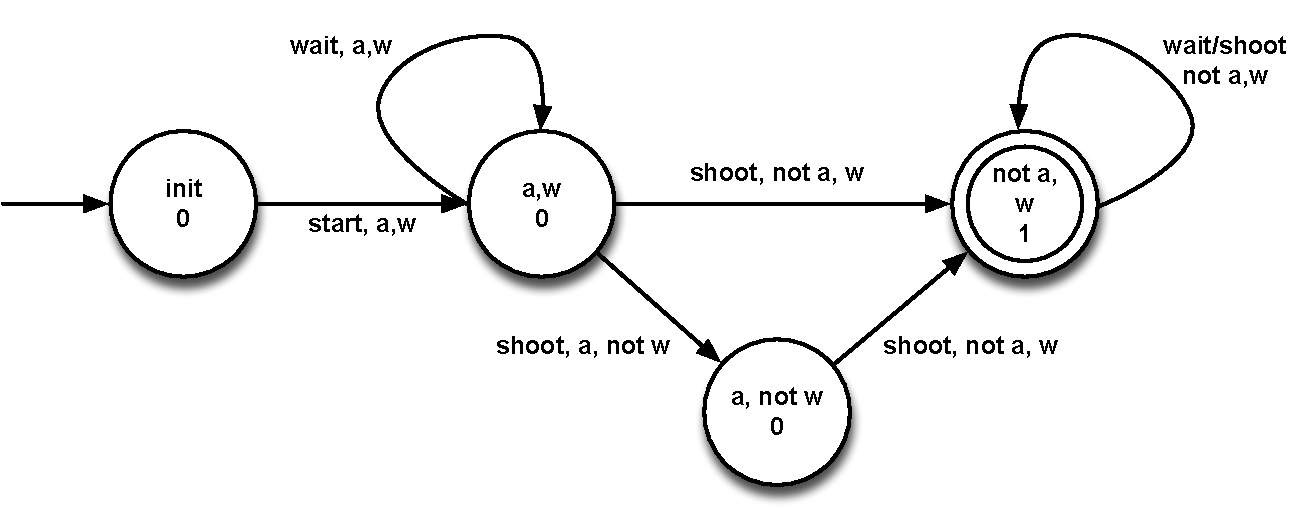
\includegraphics[width=0.7\textwidth]{images/cartesian-prod}
\caption{The \DFA automaton corresponding to $\automaton_\D \times \automaton_\varphi$} 
\label{fig:dfa-game}
\end{figure}

\noindent As we can see in Figure \ref{fig:dfa-game}, each transition reads both the action and its effect. This is not suitable for a practical implementation. Thus, we do not perform the cartesian product between the two automaton. On the contrast, we build a transition system as follows:

\begin{figure}[h]
\centering
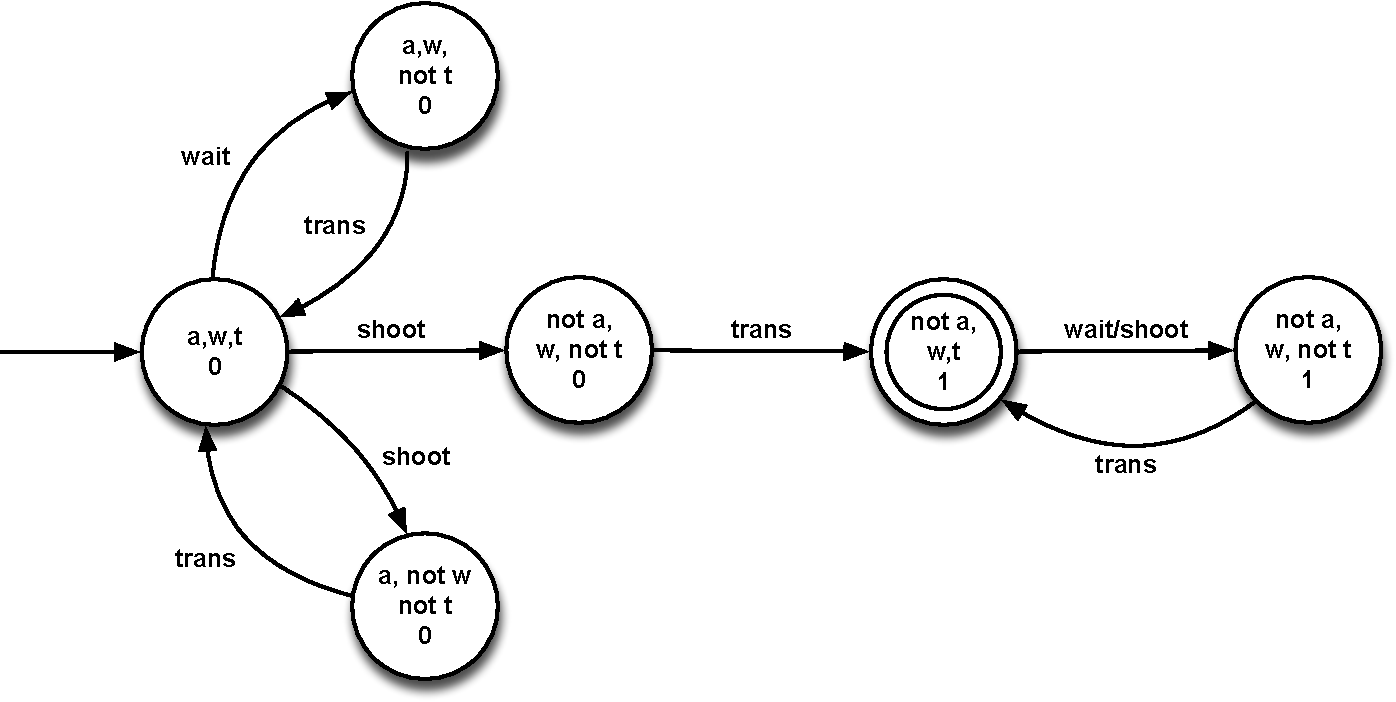
\includegraphics[width=0.8\textwidth]{images/yale-our-sol}
\caption{The \DFA automaton corresponding to $\automaton_\D \times \automaton_\varphi$} 
\label{fig:yale-our-sol}
\end{figure}

\end{example}

The transition system, shown in Figure \ref{fig:yale-our-sol}, expresses the new domain $\D'$ that has a perfect alternation of transitions. In particular, actions of the initial domain $\D$ alternates with a special action, that we called \texttt{trans}, representing the movement done by $\automaton_\varphi$. 

In the next Section, we will explain how the new domain $\D'$ and the new problem $\P'$ can be written in \PDDL by showing the encoding of \LTLf/\PLTL goals in \PDDL.

\subsection{Encoding of \LTLf/\PLTL goals in \PDDL}
In this Section, we describe the process of obtaining the new domain $\D'$ and the new problem $\P'$, both specified in \PDDL. Both the original \PDDL domain $\D$ and problem $\P$ change when introducing \LTLf/\PLTL goals. Regarding the original domain $\D$, we have the following:
\begin{itemize}
\item 
\end{itemize}

























\section{Implementation}\label{sec:planning-implementation}
\subsection{Package Structure}
\subsection{\PDDL}
\subsection{Automa}
\subsection{Main Module}
\section{Results}
\section{Summary}
